\documentclass[a4paper]{article}
\usepackage{times}
\usepackage{mathptmx}
\usepackage[boldfont,slantfont]{xeCJK}
\setmainfont{Times New Roman}
\setsansfont{Times New Roman}
\setCJKmainfont{宋体}
\setCJKsansfont{黑体}
\setCJKmonofont{仿宋}
\setCJKfamilyfont{hei}{黑体}
\setCJKfamilyfont{kai}{楷体}
\newcommand{\hei}{\CJKfamily{hei}}
\newcommand{\kai}{\CJKfamily{kai}}
\usepackage{amsmath,amssymb,amsthm}
\usepackage{geometry}
\geometry{left=2.5cm,right=2.5cm,top=2.5cm,bottom=2.5cm}
\usepackage{fancyhdr}
\usepackage{lastpage}
\usepackage{pgf,tikz}
\usetikzlibrary{calc,intersections}
\usetikzlibrary{arrows,snakes,backgrounds}
\usetikzlibrary{shapes.geometric}
\pgfmathdeclarefunction{fix}{1}{\global \pgfmathunitsdeclaredfalse}
\usepackage{array}
\def\bkh{\!\!(}
\def\ekh{)\!\!}
\def\dh{、\!\!}
\def\dou{,\!\!}
\def\mao{:\!\!}
\def\fen{;\!\!}
\def\wen{?\!\!}
\def\leq{\leqslant}
\def\geq{\geqslant}
\newcommand{\tabincell}[2]{\begin{tabular}{@{}#1@{}}#2\end{tabular}}
\begin{document}
    \renewcommand{\baselinestretch}{1.25}\normalsize
    \setlength{\parindent}{2em}
    \setlength{\abovedisplayskip}{1pt}
    \setlength{\belowdisplayskip}{1pt}
    \pagestyle{fancy}
    \fancyhf{}
    \fancyhead[l]{NOIP提高班——数学专项练习}
    \fancyhead[r]{2018年2月22日}
    \fancyfoot[c]{第\thepage 页\qquad 共\pageref{LastPage} 页}
    \renewcommand{\headrulewidth}{0.1mm}
    
    \begin{center}
        {\LARGE \hei NOIP提高班——数学专项练习}

        \vspace*{1mm}

        {\kai \bkh 请选手务必仔细阅读本页内容\ekh}
    \end{center}

    {\hei 一\dh 题目概况}

    \begin{center}
        \begin{tabular}{|*{4}{p{3.5cm}<{\centering}|}}
            \hline
            中文题目名称 & 哈希函数 & 仪仗队 & 贺卡 \\\hline
            英文题目与子目录名 & hash & honourguard & card \\\hline
            可执行文件名 & hash & honourguard & card \\\hline
            输入文件名 & hash.in & honourguard.in & card.in \\\hline
            输出文件名 & hash.out & honourguard.out & card.out \\\hline
            每个测试点时限 & 1秒 & 2秒 & 3秒 \\\hline
            测试点数目 & 10 & 10 & 10 \\\hline
            每个测试点分值 & 10 & 10 & 10 \\\hline
            附加样例文件 & 有 & 有 & 有 \\\hline
            结果比较方式 & \multicolumn{3}{c|}{全文比较\bkh 过滤行末空格和文末回车\ekh} \\\hline
            题目类型 & 传统 & 传统 & 传统 \\\hline
            运行内存上限 & 256M & 1G & 256M \\\hline
        \end{tabular}
    \end{center}

    {\hei 二\dh 提交源程序文件名}

    \begin{center}
        \begin{tabular}{|*{4}{p{3.5cm}<{\centering}|}}
            \hline
            对于 \makebox[28pt][l]{C++}语言 & hash.cpp & honourguard.cpp & card.cpp \\\hline
            对于 \makebox[28pt][l]{C}语言 & hash.c & honourguard.c & card.c \\\hline
            对于 \makebox[28pt][l]{Pascal}语言 & hash.pas & honourguard.pas & card.pas \\\hline
        \end{tabular}
    \end{center}

    {\hei 三\dh 编译命令\bkh 不包含任何优化开关\ekh}

    \begin{center}
        \begin{tabular}{|*{4}{p{3.5cm}<{\centering}|}}
            \hline
            对于 \makebox[28pt][l]{C++}语言 & g++ -o hash hash.cpp -lm & g++ -o honourguard honourguard.cpp -lm & g++ -o card card.cpp -lm \\\hline
            对于 \makebox[28pt][l]{C}语言 & gcc -o hash hash.c -lm & gcc -o honourguard honourguard.c -lm & gcc -o card card.c -lm \\\hline
            对于 \makebox[28pt][l]{Pascal}语言 & fpc hash.pas & fpc honourguard.pas & fpc card.pas \\\hline
        \end{tabular}
    \end{center}

    {\hei 注意事项\mao}

    1. 文件名\bkh 程序名和输入输出文件名\ekh 必须使用英文小写\fen

    2. C/C++中函数main()的返回值类型必须是int\dou 程序正常结束时的返回值必须是0\fen

    3. 只提供Linux格式附加样例文件.

    \newpage

    \begin{center}
        \Large \hei 1. 哈希函数

        {\ttfamily (hash.cpp/c/pas)}
    \end{center}

    【问题描述】

    明明觉得hash是个好算法\dou 代码短\dh 效率高. 某天\dou 他碰到了一个求正方形个数的问题\dou 于是很淡定地枚举对角线\dou 然后用hash判存在\dou 妥妥的搞定\dou 但是提交后却wa了几个点. 仔细观察其hash函数为\mao $h=xy+x+y$. 为了让明明知道这个函数存在什么问题\dou 对于给出的一个$h$值\dou 请你来告诉他有多少对$(x,y)$满足上述式子\bkh $\max\{x,y\}\leq h$\fen$h,x,y$都为非负整数\ekh\wen

    【输入格式】

    输入文件名为{\ttfamily hash.in}.

    输入文件第一行包含一个正整数$T$\dou 表示数据组数.

    接下来$T$行每行包含一个整数$h$\dou 意义详见题目描述.

    【输出格式】

    输出文件名为{\ttfamily hash.out}.

    输出文件包含$T$行\dou 每行一个整数\dou 分别表示有多少组$(x,y)$满足要其对应的$h$值.

    【输入输出样例1】

    \begin{tabular}{|*{2}{p{5cm}|}}
        \hline
        {\ttfamily hash.in} & {\ttfamily hash.out} \\\hline
        \tabincell{l}{3\\1\\3\\4} & \tabincell{l}{2\\3\\2\\~~} \\\hline
    \end{tabular}

    【输入输出样例1说明】

    第一组\fen $(1,0),(0,1)$.

    第二组\fen $(0,3),(1,1),(3,0)$.

    第三组\fen $(4,0),(0,4)$.

    【输入输出样例2】

    见选手目录下的{\ttfamily hash/hash2.in}和{\ttfamily hash/hash2.ans}.

    【数据规模与约定】

    对于30\% 的数据\dou $h\leq 2,000$\dou $T\leq 1,000$.

    对于70\% 的数据\dou $h\leq 10,000$\dou $T\leq 10,000$.

    对于100\% 的数据\dou $h\leq {10}^8$\dou $T\leq 10,000$.

    \newpage

    \begin{center}
        \Large \hei 2. 仪仗队

        {\ttfamily (honourguard.cpp/c/pas)}
    \end{center}

    【问题描述】

    作为体育委员\dou C君负责这次运动会仪仗队的训练. 仪仗队是由学生组成的$N\times N$的方阵\dou 为了保证队伍在行进中整齐划一\dou C君会跟在仪仗队的左后方\dou 根据其视线所及的学生人数来判断队伍是否整齐\bkh 如下图\ekh . 现在\dou C君希望你告诉他队伍整齐时能看到的学生人数.

    \begin{center}
        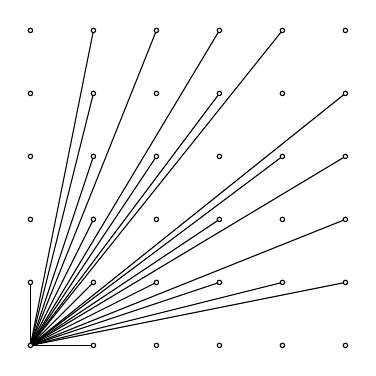
\begin{tikzpicture}[scale=0.8]
            \draw (0,0)--(1,0);
            \draw (0,0)--(0,1);
            \draw (0,0)--(1,1);
            \draw (0,0)--(2,1);
            \draw (0,0)--(3,1);
            \draw (0,0)--(4,1);
            \draw (0,0)--(5,1);
            \draw (0,0)--(1,2);
            \draw (0,0)--(3,2);
            \draw (0,0)--(5,2);
            \draw (0,0)--(1,3);
            \draw (0,0)--(2,3);
            \draw (0,0)--(4,3);
            \draw (0,0)--(5,3);
            \draw (0,0)--(1,4);
            \draw (0,0)--(3,4);
            \draw (0,0)--(5,4);
            \draw (0,0)--(1,5);
            \draw (0,0)--(2,5);
            \draw (0,0)--(3,5);
            \draw (0,0)--(4,5);
            \foreach \x in {0,1,...,5}
                \foreach \y in {0,1,...,5}
                    \draw [fill=white] (\x,\y) circle (1pt);
        \end{tikzpicture}
    \end{center}

    【输入格式】

    输入文件名为{\ttfamily honourguard.in}.

    输入数据仅一行\dou 包含一个正整数$N$\dou 表示方阵的边长.

    【输出格式】

    输出文件名为{\ttfamily honourguard.out}.

    输出数据仅一行\dou 包含一个正整数$M$\dou 为C君应看到的学生人数.

    【输入输出样例1】

    \begin{tabular}{|*{2}{p{5cm}|}}
        \hline
        {\ttfamily honourguard.in} & {\ttfamily honourguard.out} \\\hline
        4 & 9 \\\hline
    \end{tabular}

    【输入输出样例1说明】

    \begin{center}
        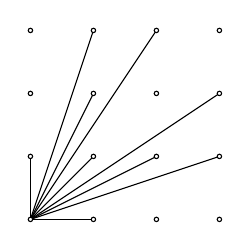
\begin{tikzpicture}[scale=0.8]
            \draw (0,0)--(1,0);
            \draw (0,0)--(0,1);
            \draw (0,0)--(1,1);
            \draw (0,0)--(2,1);
            \draw (0,0)--(3,1);
            \draw (0,0)--(1,2);
            \draw (0,0)--(3,2);
            \draw (0,0)--(1,3);
            \draw (0,0)--(2,3);
            \foreach \x in {0,1,2,3}
                \foreach \y in {0,1,2,3}
                    \draw [fill=white] (\x,\y) circle (1pt);
        \end{tikzpicture}
    \end{center}

    【输入输出样例2】

    见选手目录下的{\ttfamily honourguard/honourguard2.in}和{\ttfamily honourguard/honourguard2.ans}.

    【数据规模与约定】

    对于30\%的数据\dou $1\leq N\leq 1,000$.

    对于70\%的数据\dou $1\leq N\leq 40,000$.

    对于100\%的数据\dou $1\leq N\leq 40,000,000$.

    \newpage

    \begin{center}
        \Large \hei 3. 贺卡

        {\ttfamily (card.cpp/c/pas)}
    \end{center}

    【问题描述】

    过年了\dou zzy和她的同学共$N$人互相送贺卡. 他们每人写了一张贺卡并送给了另外一名同学\dou 而每个同学恰好收到一张贺卡. 问满足条件的送贺卡方式有多少种\wen

    【输入格式】

    输入文件名为{\ttfamily card.in}.

    输入数据仅一行\dou 包含一个正整数$N$\dou 表示同学的总人数.

    【输出格式】

    输出文件名为{\ttfamily card.out}.

    输出数据仅一行\dou 包含一个正整数\dou 为满足条件的方案数.

    {\hei 由于答案可能很大\dou 请输出其对${10}^9+7$取模的结果.}

    【输入输出样例1】

    \begin{tabular}{|*{2}{p{5cm}|}}
        \hline
        {\ttfamily card.in} & {\ttfamily card.out} \\\hline
        4 & 9 \\\hline
    \end{tabular}

    【输入输出样例1说明】

    我们把三名同学编号为$1,2,3$\dou 我们用$x\to y$表示$x$同学的贺卡送给了$y$同学.

    $(1)$ $1\to 2,2\to 1,3\to 4,4\to 3$\fen

    $(2)$ $1\to 3,2\to 4,3\to 1,4\to 2$\fen

    $(3)$ $1\to 4,2\to 3,3\to 2,4\to 1$\fen

    $(4)$ $1\to 2,2\to 3,3\to 4,4\to 1$\fen

    $(5)$ $1\to 2,2\to 4,3\to 1,4\to 3$\fen

    $(6)$ $1\to 3,2\to 4,3\to 2,4\to 1$\fen

    $(7)$ $1\to 3,2\to 1,3\to 4,4\to 2$\fen

    $(8)$ $1\to 4,2\to 3,3\to 1,4\to 2$\fen

    $(9)$ $1\to 4,2\to 1,3\to 2,4\to 3$.

    【输入输出样例2】

    见选手目录下的{\ttfamily card/card2.in}和{\ttfamily card/card2.ans}.

    【数据规模与约定】

    对于20\% 的数据\dou $N\leq 8$.

    对于100\% 的数据\dou $N\leq {10}^8$.
\end{document}